\documentclass[a4paper,11pt]{article}
\usepackage[utf8]{inputenc}
\usepackage{geometry}
\geometry{margin=2.5cm}
\usepackage{amsmath, amssymb, amsfonts}
\usepackage{graphicx}
\usepackage{float}
\usepackage{hyperref}
\usepackage{subcaption}
\usepackage{physics}
\usepackage{booktabs}

\title{Simulation of String Oscillations using the Velocity Verlet Method}
\author{Tomasz Karpiński}
\date{\today}

\begin{document}

\maketitle

\section{Introduction}
The objective of this project is to simulate the dynamics of a one-dimensional massive string. The physical system is governed by the wave equation, augmented with terms for frictional damping and external driving forces. The vertical displacement of the string $u(x,t)$ evolves according to the partial differential equation:

\begin{equation}
    \frac{\partial^2 u}{\partial t^2} = c^2 \frac{\partial^2 u}{\partial x^2} - \gamma \frac{\partial u}{\partial t} + F_{ext} \sin(\Omega t) \delta(x - x_p)
    \label{eq:wave}
\end{equation}

where $c = \sqrt{T/\rho}$ is the speed of sound (with tension $T$ and linear mass density $\rho$), $\gamma$ is the damping coefficient, and the last term represents a periodic external force applied at a specific point $x_p$.

We investigate various scenarios, including reflection at boundaries, propagation of wave packets, impedance mismatch in non-homogeneous media, spectral decomposition of modes, and mechanical resonance.

\section{Numerical Method}

\subsection{Mesh, finite difference method, discretization}
To simulate the wave dynamics numerically, the continuous string of length $L$ is approximated by a discrete grid of points. We divide the spatial domain into $N$ equidistant nodes, resulting in a spatial resolution defined by:
\begin{equation}
    \Delta x = \frac{L}{N-1}, \quad x_i = \Delta x \cdot i, \quad i = 0, 1, 2, \dots, N-1
\end{equation}
Similarly, the time evolution is discretized into steps of size $\Delta t$:
\begin{equation}
    t_n = \Delta t \cdot n, \quad n = 0, 1, 2, \dots
\end{equation}
To ensure numerical stability, the time step is coupled to the spatial step via the Courant-Friedrichs-Lewy (CFL) condition. We utilize a safety factor $\alpha \le 1$ (specifically $\alpha = 0.5$) to define:
\begin{equation}
    \Delta t = \alpha \frac{\Delta x}{c}
\end{equation}
Using the notation $u_i^n$ for displacement and $v_i^n$ for velocity at node $i$ and time $n$, the discrete form of the driven, damped wave equation is given by:
\begin{equation}
    a_i^n = c_i^2 \frac{u_{i+1}^n - 2u_i^n + u_{i-1}^n}{\Delta x^2} - \gamma v_i^n + F_{ext} \sin(\Omega t_n)\delta_{i,i_p}
\end{equation}

\subsection{Boundary conditions (BC)}
The behavior of the wave at the string's extremities is governed by boundary conditions. We investigate two distinct physical scenarios:
\begin{itemize}
    \item \textit{Fixed BC}: Corresponds to a Dirichlet condition where the endpoints are clamped and cannot move.
    \begin{equation}
        u(0, t) = u(L, t) = 0 \implies u_0^n = u_{N-1}^n = 0
    \end{equation}
    \item \textit{Open BC}: Corresponds to a Neumann condition where the derivative is zero, implying the ends are free to slide transversely.
    \begin{equation}
        \frac{\partial u}{\partial x}\bigg|_{x=0,L} = 0 \implies u_0^n \leftarrow u_1^n \text{ and } u_{N-1}^n \leftarrow u_{N-2}^n
    \end{equation}
\end{itemize}
Note that for the open boundary implementation, we update the ghost nodes based on their neighbors, and explicit velocity calculations at these boundaries are not required for the algorithm.

\subsection{Kinetic and potential energies}
In a lossless system, the total mechanical energy is an invariant of motion. Monitoring this quantity serves as a crucial validation of the numerical scheme's stability. The total kinetic energy is computed by summing the contributions of all moving internal mass elements:
\begin{equation}
    E_{kin}(t_n) = \sum_{i=1}^{N-2} \frac{m_i (v_i^n)^2}{2} = \sum_{i=1}^{N-2} \frac{\Delta x \rho_i (v_i^n)^2}{2}
\end{equation}
The potential energy arises from the elastic stretching of the string segments. Using a backward difference approximation for the gradient, we integrate the tension work along the string:
\begin{equation}
    E_{pot}(t_n) = \sum_{i=1}^{N-1} \frac{\Delta x T}{2} \left( \frac{\partial u}{\partial x}\bigg|_{x=x_i} \right)^2 = \sum_{i=1}^{N-1} \frac{\Delta x T}{2} \left( \frac{u_i^n - u_{i-1}^n}{\Delta x} \right)^2
\end{equation}
As noted in the reference method, the summation indices for potential energy run from $1$ to $N-1$ due to the spatial derivative stencil used.

\subsection{Velocity Verlet method}
We employ the Velocity Verlet integration scheme, a symplectic algorithm favoured for its energy conservation properties in oscillatory systems. The state update from step $t$ to $t+\Delta t$ proceeds as follows:
\begin{enumerate}
    \item \textbf{Time update:} Increment simulation time.
    \item $t \leftarrow (it - 1) \cdot \Delta t$
    \item \textbf{Initial Acceleration:} Compute forces based on current configuration.
    \item $a_i \leftarrow c_i^2 \frac{u_{i+1}-2u_i+u_{i-1}}{\Delta x^2} - \gamma \cdot v_i + F_{ext} \sin(\Omega t) \cdot \delta_{i,i_p}, \quad i = 1, 2, \dots, N - 2$
    \item \textbf{Half-step Velocity:} Predict velocity at the midpoint $t + \Delta t/2$.
    \begin{equation}
        \tilde{v}_i \leftarrow v_i + \frac{\Delta t}{2} a_i, \quad i = 1, 2, \dots, N - 2
    \end{equation}
    \item \textbf{Position Update:} Advance positions using the half-step velocity.
    \begin{equation}
        u_i \leftarrow u_i + \tilde{v}_i \Delta t
    \end{equation}
    \item \textbf{Apply Boundary Conditions:} Enforce constraints on the new positions.
    \begin{itemize}
        \item $u_0 \leftarrow 0$ and $u_{N-1} \leftarrow 0$ for \textit{fixed BC}
        \item OR
        \item $u_0 \leftarrow u_1$ and $u_{N-1} \leftarrow u_{N-2}$ for \textit{open BC}
    \end{itemize}
    \item \textbf{New Acceleration:} Recalculate forces at $t + \Delta t$ using the new displacements $u$ and the half-step velocities $\tilde{v}$ (for the damping term).
    \begin{equation}
        a_i \leftarrow c_i^2 \frac{u_{i+1}-2u_i+u_{i-1}}{\Delta x^2} - \gamma \cdot \tilde{v}_i + F_{ext} \sin(\Omega(t + \Delta t)) \cdot \delta_{i,i_p}, \quad i = 1, 2, \dots, N - 2
    \end{equation}
    \item \textbf{Full-step Velocity:} Correct the velocity to the end of the step.
    \begin{equation}
        v_i \leftarrow \tilde{v}_i + a_i \frac{\Delta t}{2}, \quad i = 1, 2, \dots, N - 2
    \end{equation}
    \item \textbf{Output:} Store $t, E_{kin}, E_{pot}$ and displacement profile $u_i$.
\end{enumerate}

\section{Results}

\subsection{Task 1: Fixed Boundary Conditions}
A Gaussian pulse is initialized at the center of a homogeneous string with fixed ends.
\begin{figure}[H]
    \centering
    \begin{subfigure}{0.48\textwidth}
        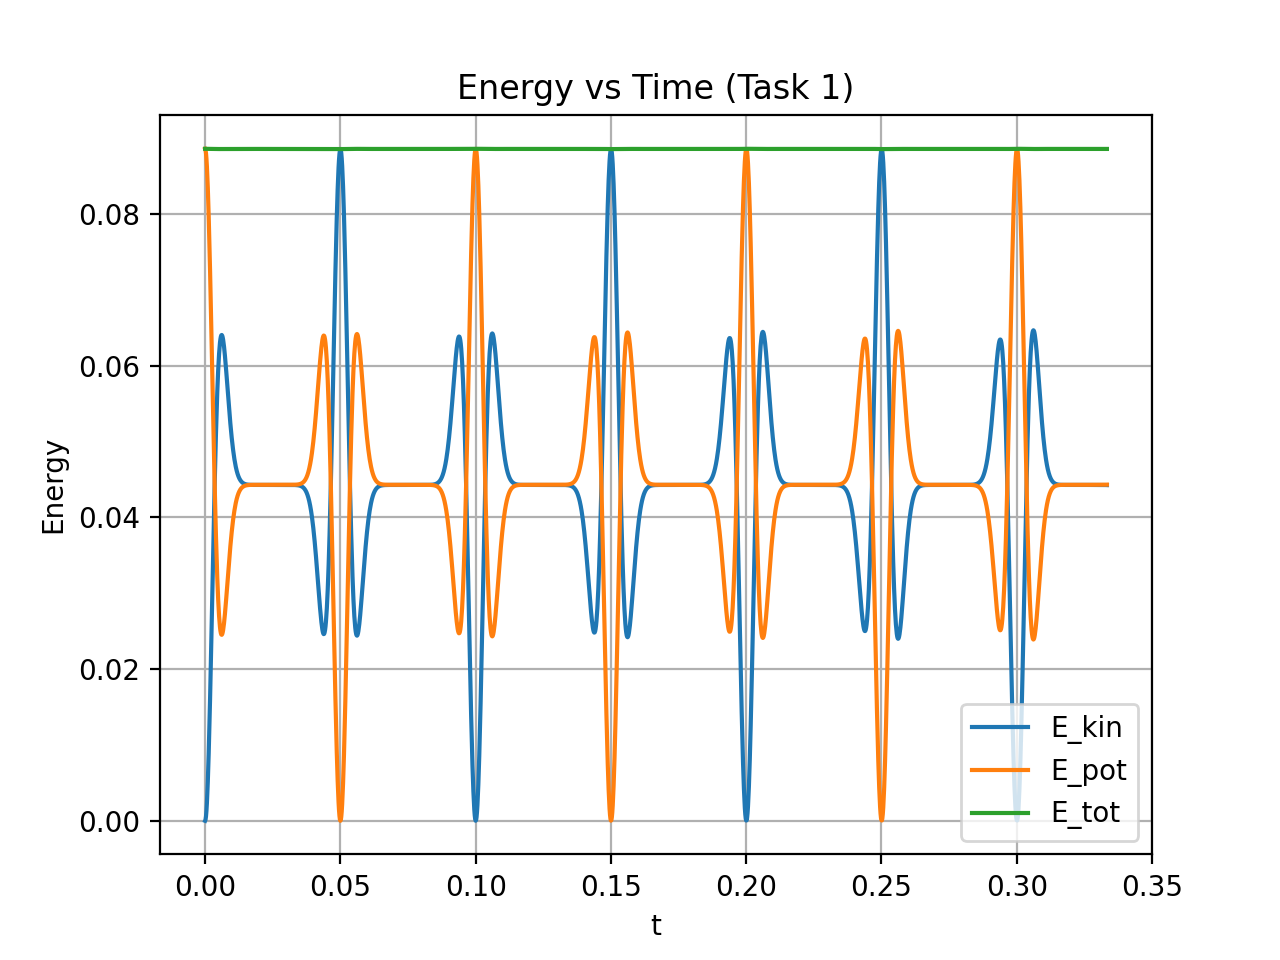
\includegraphics[width=\linewidth]{energy_task1.png}
        \caption{Energies vs Time}
    \end{subfigure}
    \begin{subfigure}{0.48\textwidth}
        
\includegraphics[width=\linewidth]{task1_displacement.png}
        \caption{Displacement Map $u(x,t)$}
    \end{subfigure}
    \caption{Task 1: The wave packet splits into two counter-propagating waves. Upon reaching the fixed boundaries, the waves reflect with an inversion of amplitude (phase shift of $\pi$), visible in the blue/red alternation in the heatmap.}
\end{figure}

\subsection{Task 2: Open Boundary Conditions}
The simulation is repeated with open (Neumann) boundary conditions.
\begin{figure}[H]
    \centering
    \begin{subfigure}{0.48\textwidth}
        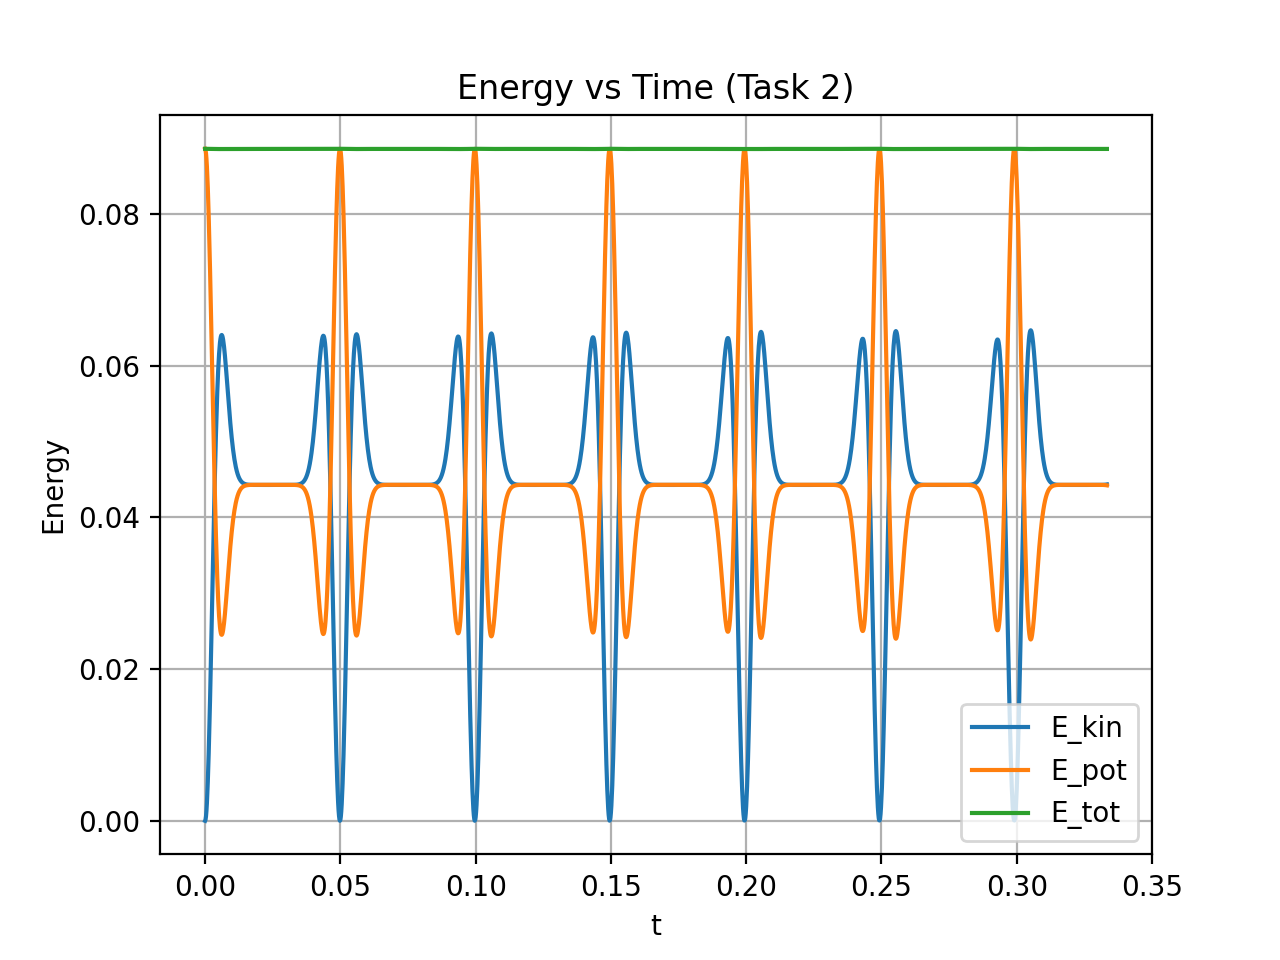
\includegraphics[width=\linewidth]{energy_task2.png}
        \caption{Energies vs Time}
    \end{subfigure}
    \begin{subfigure}{0.48\textwidth}
        
\includegraphics[width=\linewidth]{task2_displacement.png}
        \caption{Displacement Map $u(x,t)$}
    \end{subfigure}
    \caption{Task 2: Unlike the fixed case, reflection at open boundaries occurs without phase inversion. The wave maintains its sign after reflection. Total energy remains conserved (constant) in both Task 1 and 2, validating the symplectic nature of the Verlet method.}
\end{figure}

\subsection{Task 3: Moving Wave Packet}
We investigate the effect of initial velocity $v_{init}$ on wave propagation.

\subsection{Task 4: Non-homogeneous String}
The string density changes at $x=L/2$: $\rho(x > L/2) = 10\rho_0$.
\begin{figure}[H]
    \centering
    \begin{subfigure}{0.48\textwidth}
        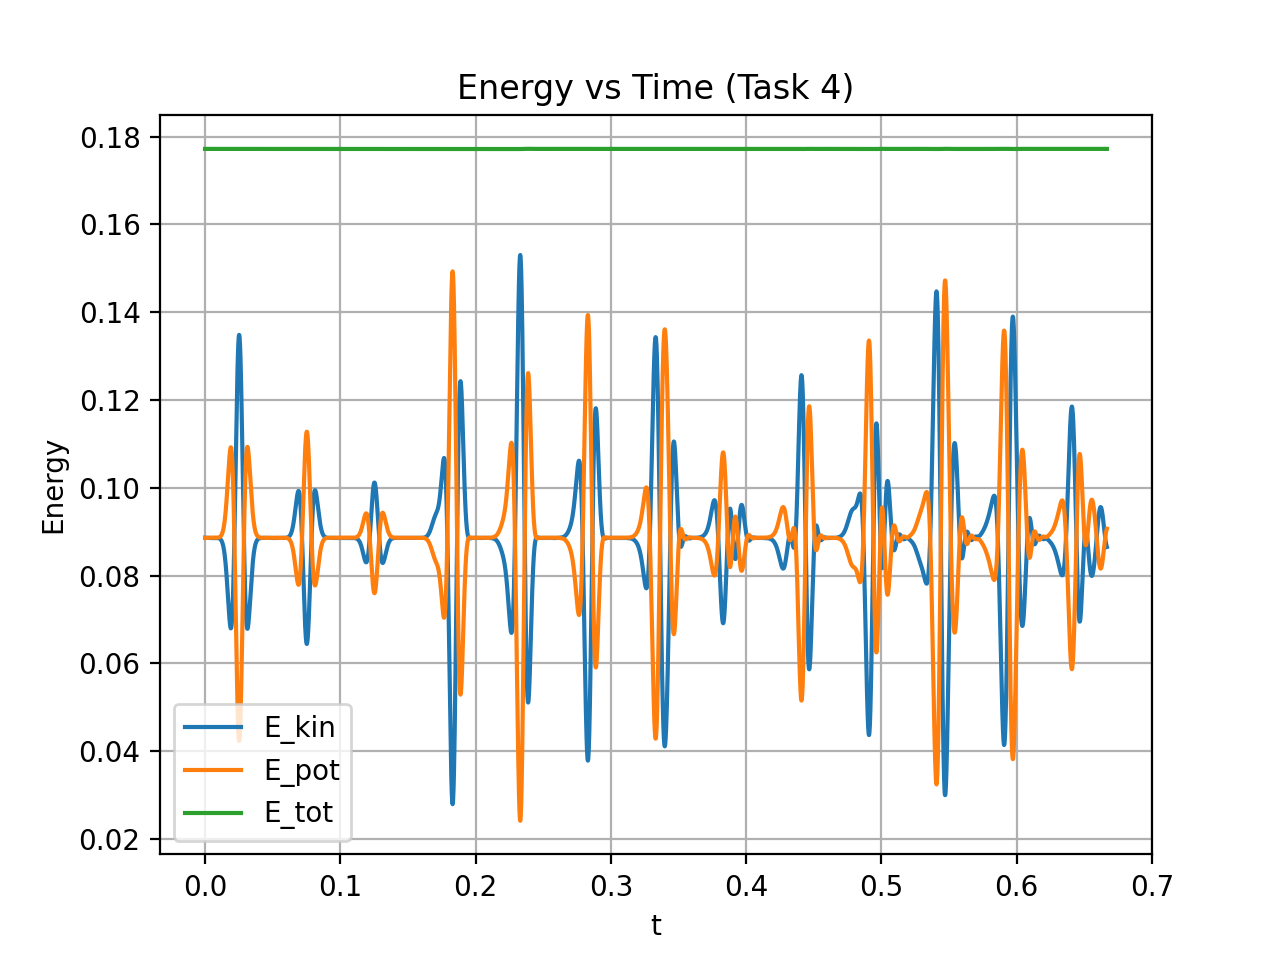
\includegraphics[width=\linewidth]{energy_task4.png}
        \caption{Energies vs Time}
    \end{subfigure}
    \begin{subfigure}{0.48\textwidth}
        
\includegraphics[width=\linewidth]{task4_displacement.png}
        \caption{Displacement Map}
    \end{subfigure}
    \caption{Task 4: An impedance mismatch occurs at the interface. Part of the wave is transmitted into the denser medium (propagating slower, as seen by the steeper slope in the space-time plot), and part is reflected. Energy is conserved.}
\end{figure}

\subsection{Task 5: Spectral Decomposition and Damping}
Friction ($\gamma = 150$) is introduced. We analyze the decay of the first three fundamental modes.
\begin{figure}[H]
    \centering
    \begin{subfigure}{0.32\textwidth}
        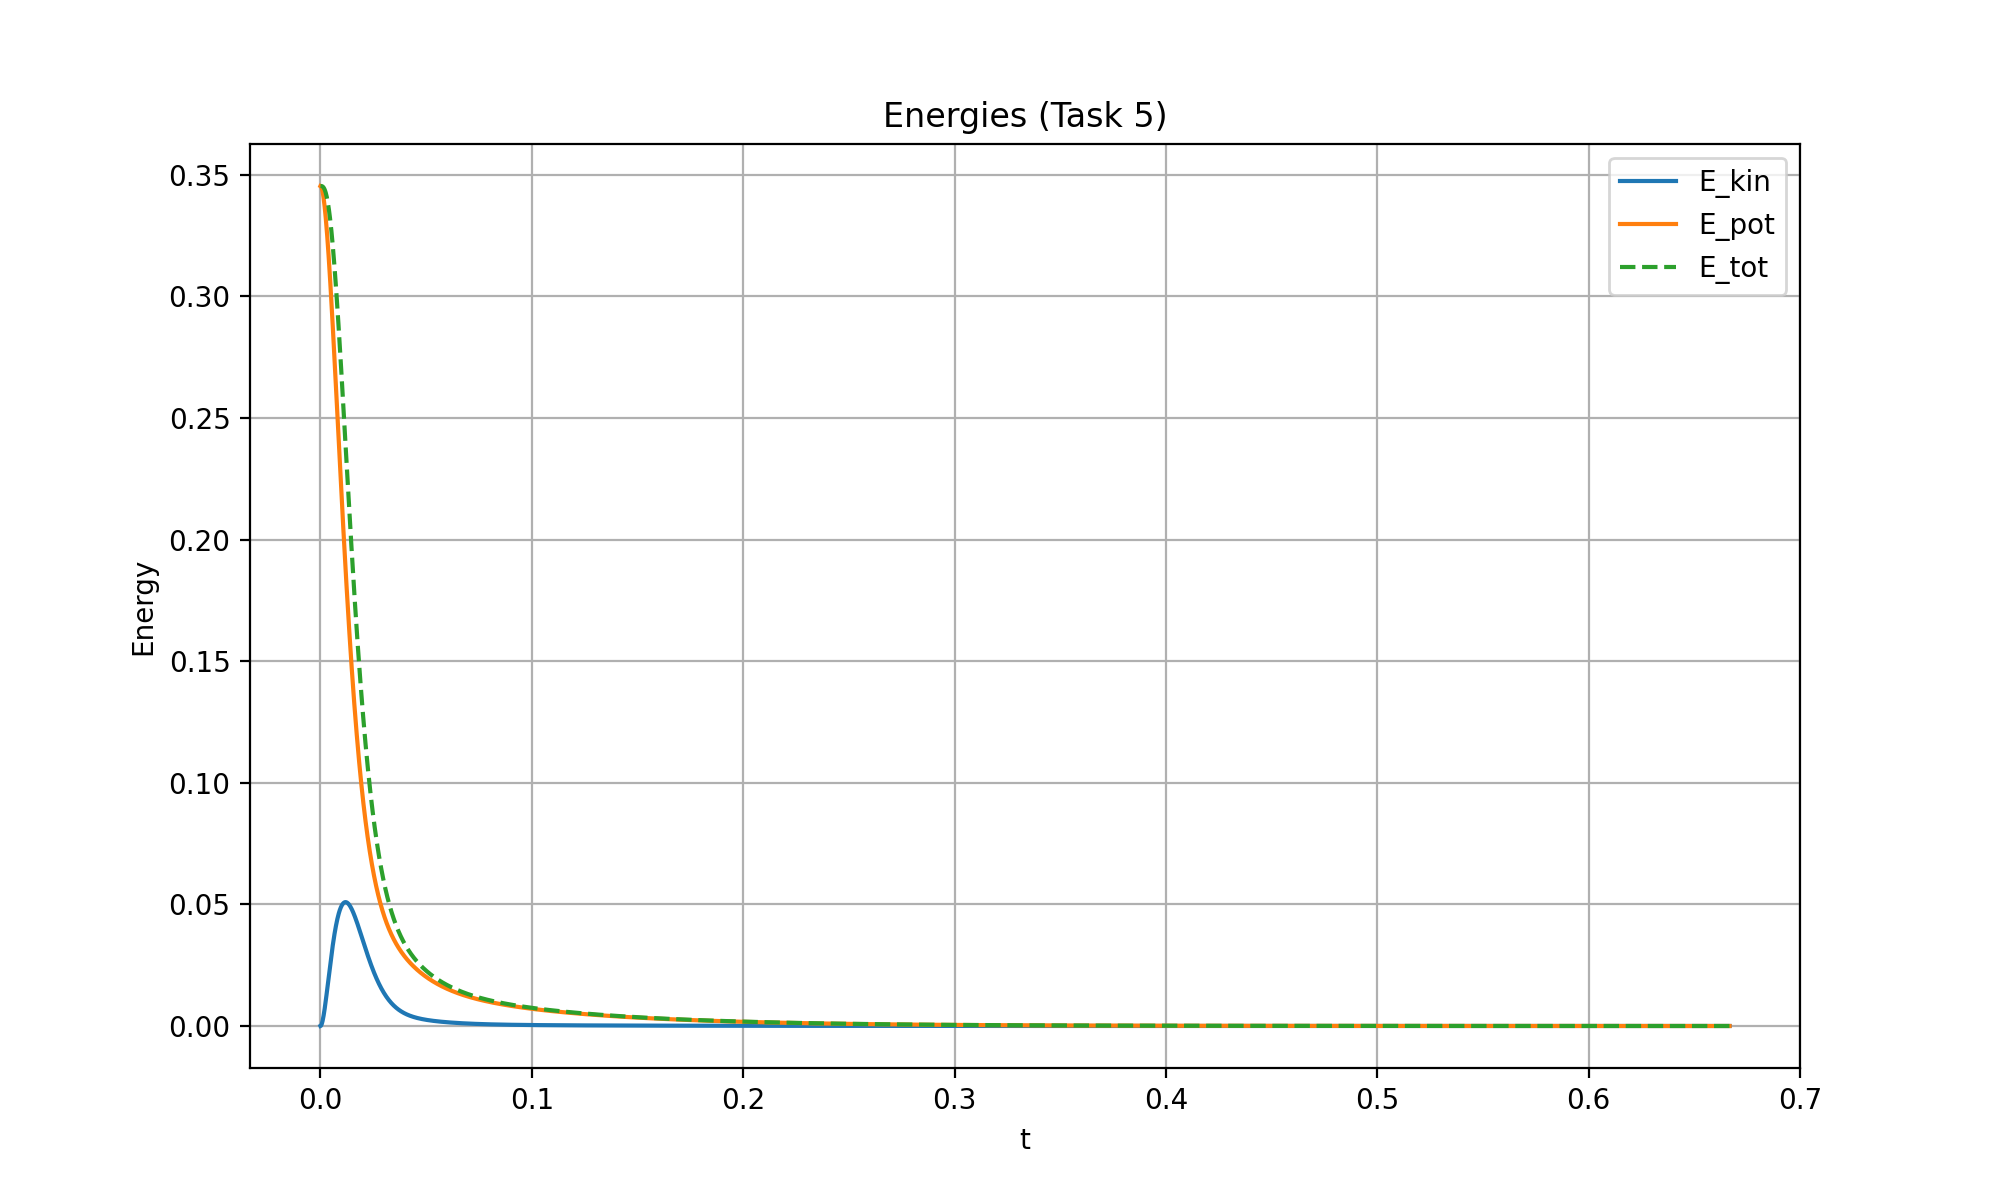
\includegraphics[width=\linewidth]{energy_task5.png}
        \caption{Energy Decay}
    \end{subfigure}
    \begin{subfigure}{0.32\textwidth}
        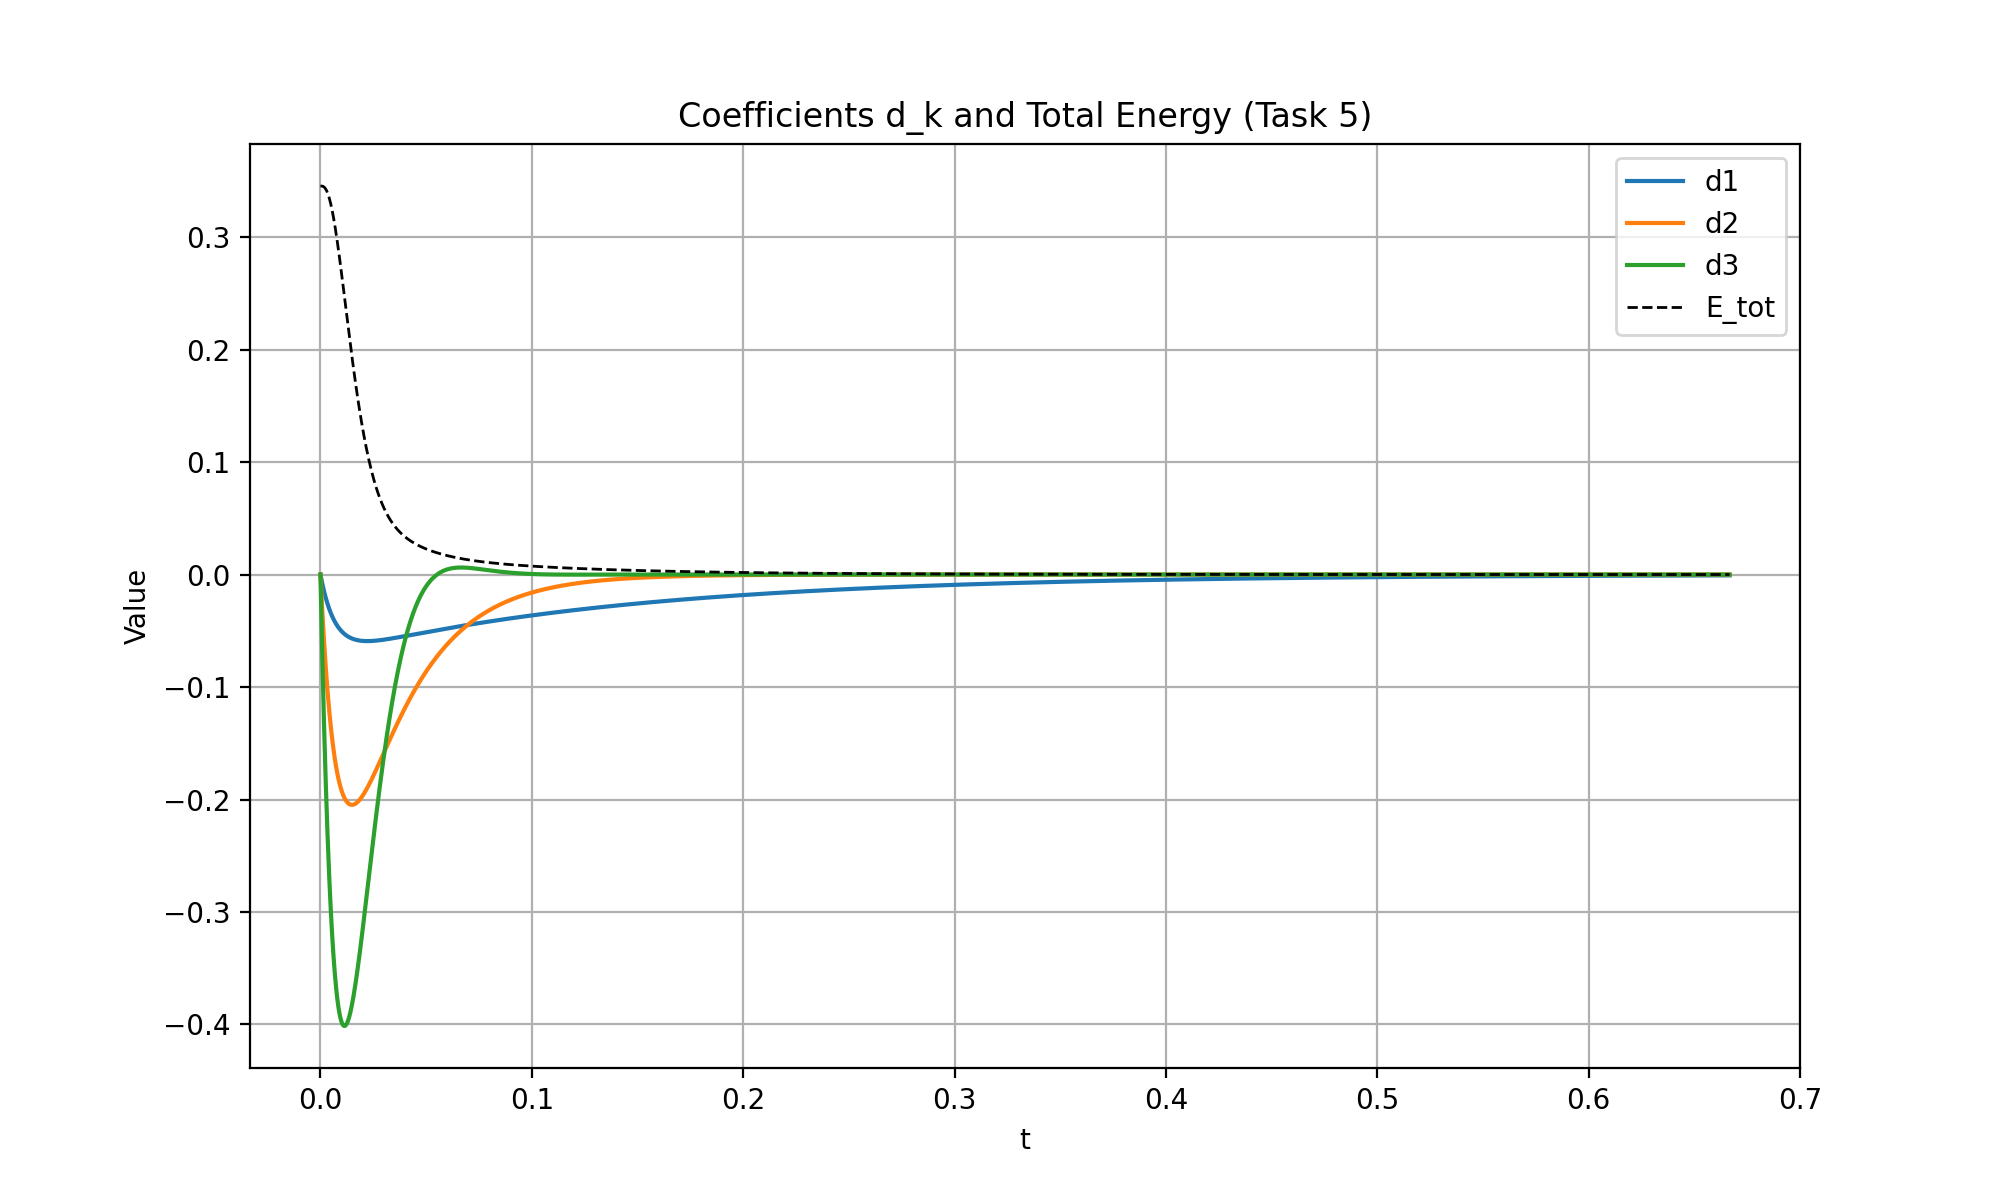
\includegraphics[width=\linewidth]{spectral_task5.png}
        \caption{Modal Coefficients}
    \end{subfigure}
    \begin{subfigure}{0.32\textwidth}
        
\includegraphics[width=\linewidth]{task5_displacement.png}
        \caption{Displacement Map}
    \end{subfigure}
    \caption{Task 5: The total energy decreases over time due to damping. Higher frequency modes decay faster than lower frequency modes, which is consistent with the physics of damped oscillations.}
\end{figure}

\subsection{Task 6: Resonance}
The string is driven by an external force $F_{ext} \sin(\Omega t)$ at point $x_p$.
\begin{figure}[H]
    \centering
    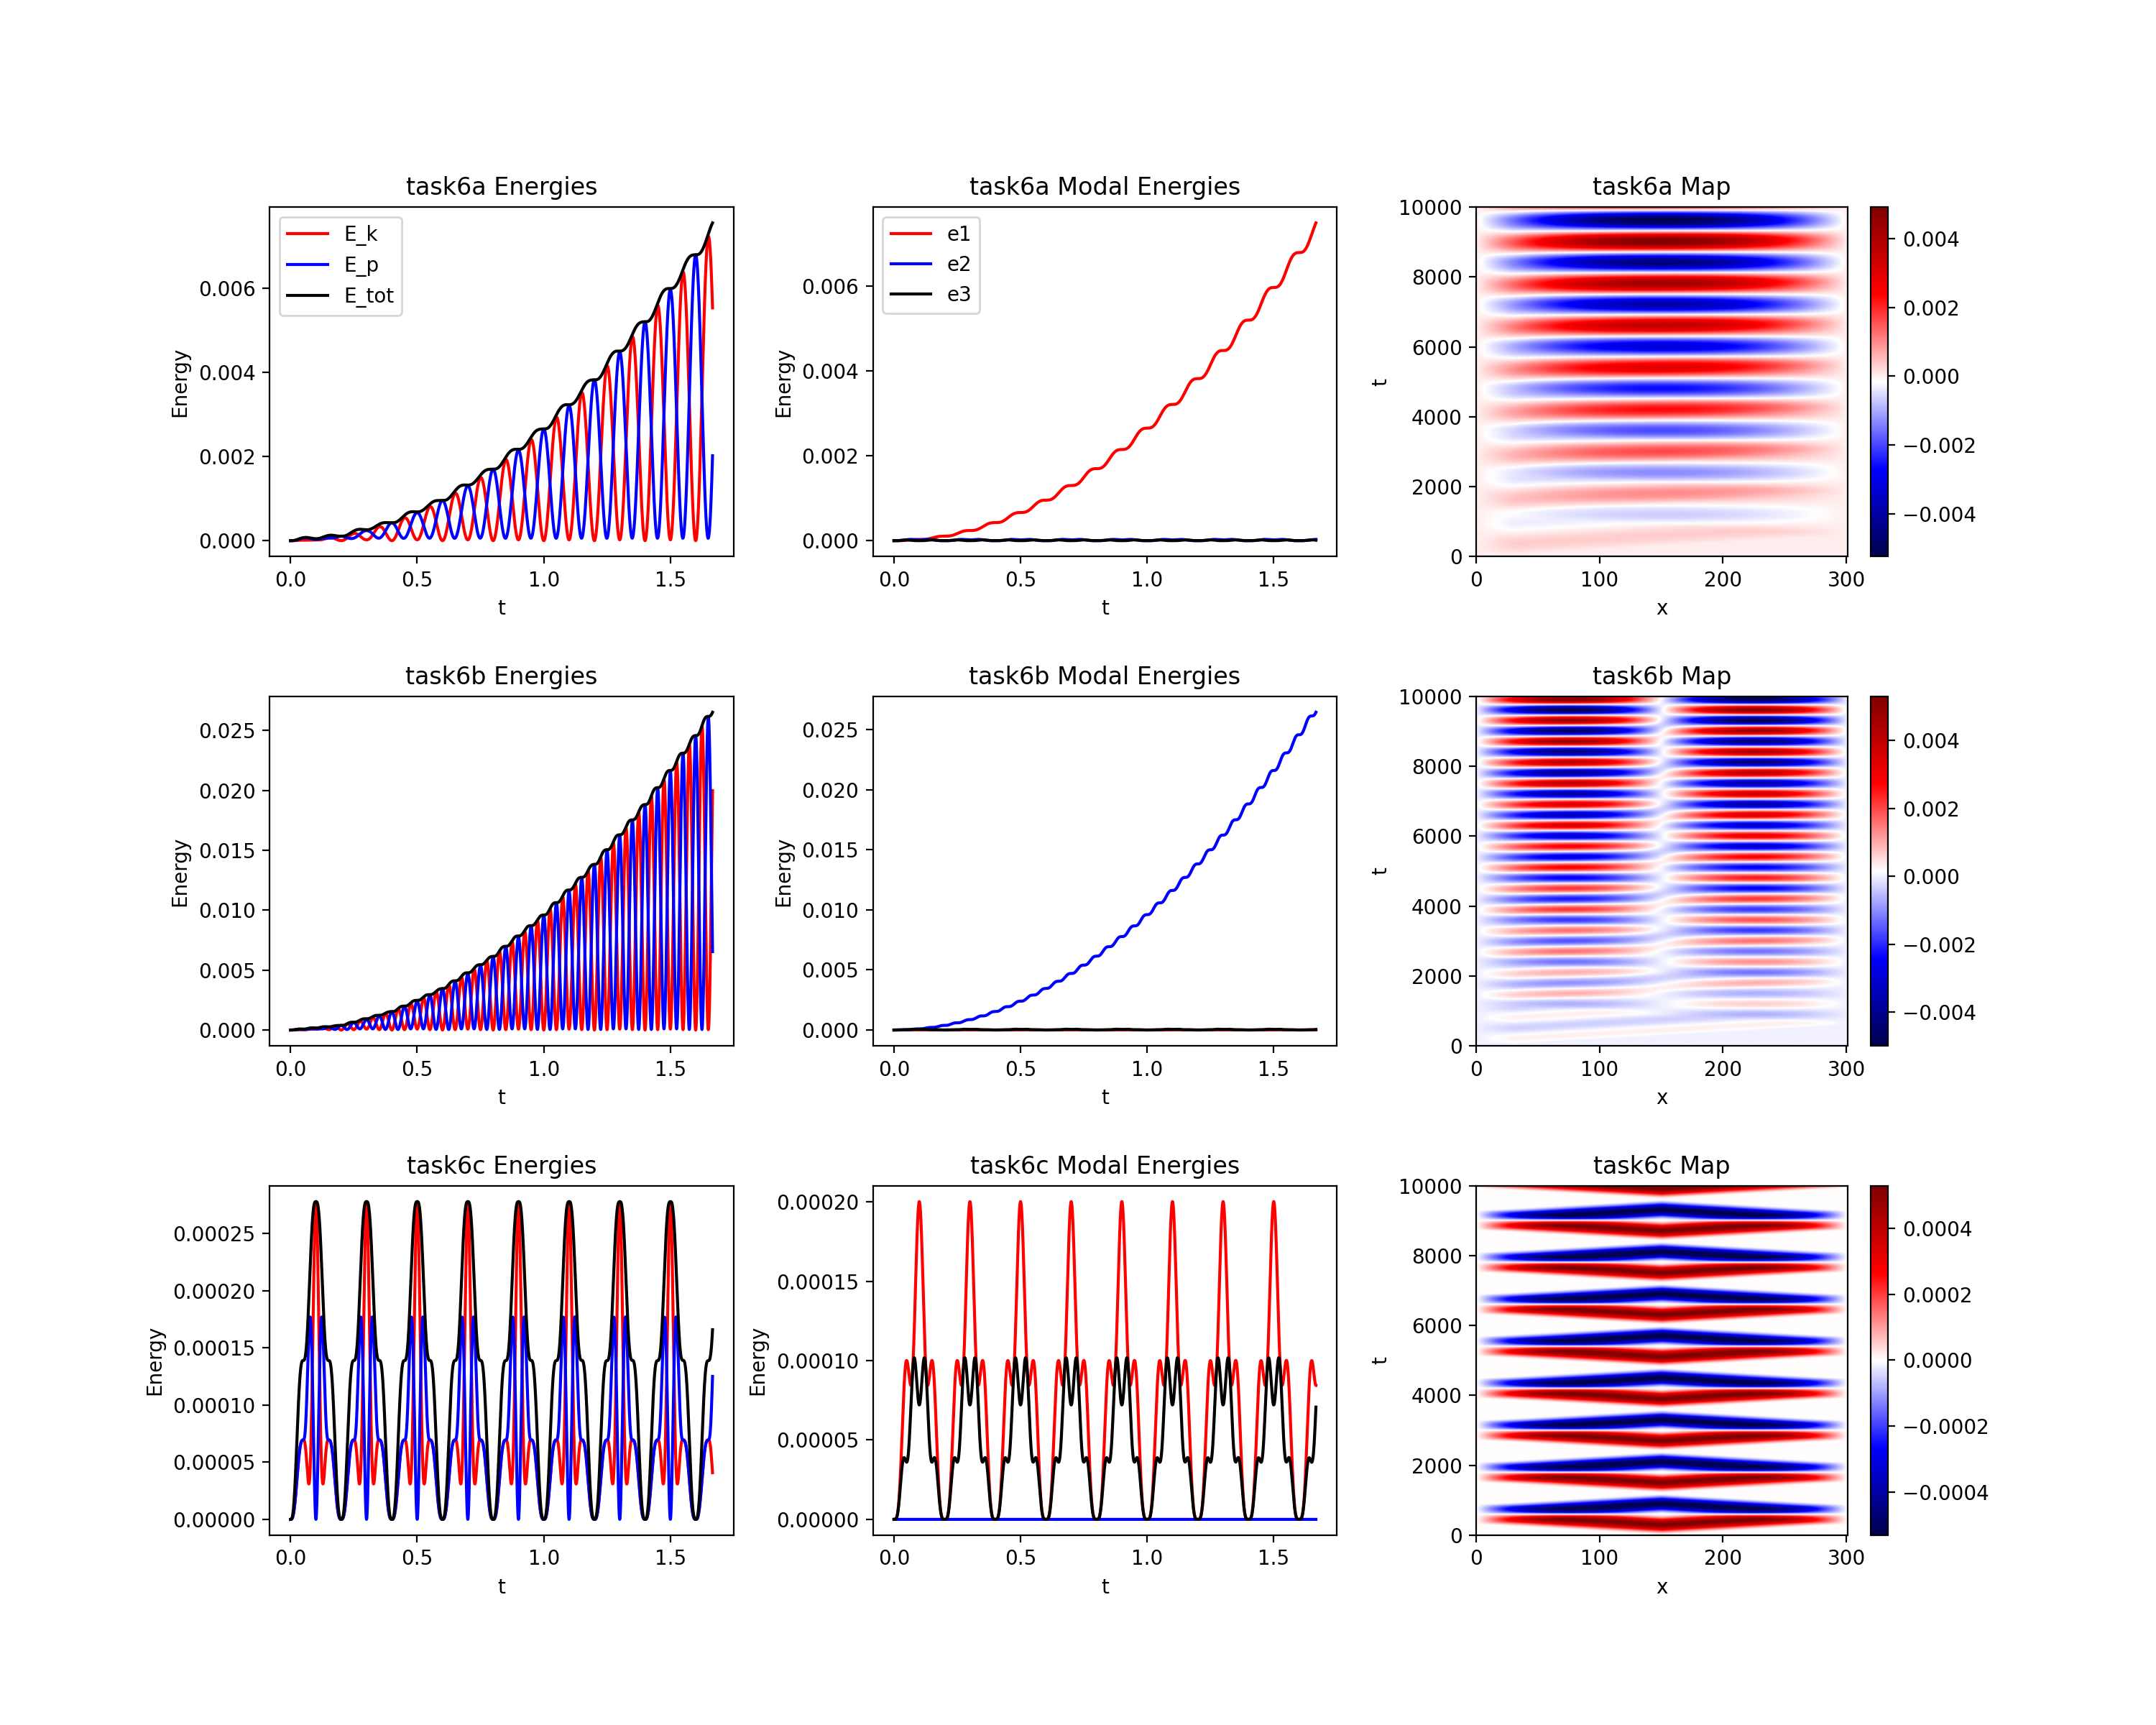
\includegraphics[width=0.95\textwidth]{task6_full_panel.png}
    \caption{Task 6: Top Row (6a): Driving at $\Omega = \omega_1$, $x_p=30$. Resonance of the 1st mode is clearly visible; energy grows quadratically. Middle Row (6b): Driving at $\Omega = \omega_2$, $x_p=30$. Resonance of the 2nd mode. Bottom Row (6c): Driving at $\Omega = \omega_2$, $x_p = (N-1)/2$ (center). The center is a node for the 2nd mode. Consequently, the force does no work, and the 2nd mode is not excited, demonstrating that resonance requires both frequency matching and spatial coupling.}
\end{figure}

\section{Conclusions}

The Velocity Verlet method proved to be a robust and stable algorithm for solving the wave equation. 

\begin{enumerate}
    \item \textbf{Conservation Laws:} In the absence of damping (Tasks 1-4), the total energy was conserved to a high degree of precision, confirming the symplectic nature of the integrator.
    \item \textbf{Boundary Conditions:} The distinction between Dirichlet (inversion) and Neumann (no inversion) boundaries was numerically verified.
    \item \textbf{Wave Propagation:} The simulation correctly reproduced the d'Alembert solution behavior, where an arbitrary pulse splits unless the initial velocity is perfectly matched to the displacement gradient ($v = -c \frac{\partial u}{\partial x}$ for right-moving).
    \item \textbf{Resonance:} The most significant observation was in Task 6. Resonance is not solely a frequency phenomenon. Even if the driving frequency matches a natural eigenfrequency ($\Omega = \omega_2$), resonance does not occur if the force is applied at a node of that standing wave mode. This highlights the importance of spatial overlap between the driving force and the mode shape.
\end{enumerate}

Overall, the project successfully demonstrated fundamental wave mechanics concepts through direct numerical simulation.

\end{document}
